% debut d'un fichier latex standard
\documentclass[a4paper,12pt,oneside]{article}
\usepackage[top=3cm, bottom=3.5cm]{geometry}
% pour l'inclusion de figures en eps,pdf,jpg,....
\usepackage{graphicx}
\usepackage{wrapfig}
\usepackage{subcaption}
\usepackage{siunitx}
% quelques symboles mathematiques en plus
\usepackage{amsmath}
% le tout en langue francaise
\usepackage[french]{babel}
\usepackage[T1]{fontenc}
% on peut ecrire directement les characteres avec l'accent
% a utiliser sur Linux/Windows
\usepackage[utf8]{inputenc}
\usepackage[rightcaption
]{sidecap}
\usepackage[export]{adjustbox}



%Pour du code non interprété
\usepackage{verbatim}
\usepackage{verbdef}% http://ctan.org/pkg/verbdef
% a utiliser sur le Mac
%\usepackage[applemac]{inputenc}
% pour l'inclusion de links dans le document (pdflatex)
\usepackage[colorlinks,bookmarks=false,linkcolor=blue,urlcolor=blue]{hyperref}
%
\usepackage{caption}
\usepackage{float}
% quelques abreviations utiles
\def \be {\begin{equation}}
\def \ee {\end{equation}}
\def \bf {\begin{figure}}
\def \ef {\end{figure}}
\def \dd  {{\rm d}}
\def \dx  {\Delta x}
\def \dt  {\Delta t}

\newcommand{\norme}[1]{\left\Vert #1 \right\Vert}
%
\newcommand{\mail}[1]{{\href{mailto:#1}{#1}}}
\newcommand{\ftplink}[1]{{\href{ftp://#1}{#1}}}



\usepackage{amssymb}








%%%%%%%%%%%%%%%%%%%%%%%%%%%%%%%%%%%%%%%%%%%%%%%%%%%%%%%%%%%%%%%%%%%%%%%%%%%%%%%%%%%%%%%%%%%%%%%%%%%%%%%%
%%%%%%%%%%%%%%%%%%%%%%%%%%%%%%%%%% le document commence ici %%%%%%%%%%%%%%%%%%%%%%%%%%%%%%%%%%%%%%%%%%%%
%%%%%%%%%%%%%%%%%%%%%%%%%%%%%%%%%%%%%%%%%%%%%%%%%%%%%%%%%%%%%%%%%%%%%%%%%%%%%%%%%%%%%%%%%%%%%%%%%%%%%%%%
\begin{document}
\pagestyle{empty}

% le titre et l'auteur
\title{Ondes : exercice 7}
\date{\today}
\author{Timothée Dao, Victor Despland\\{\small \mail{timothee.dao@epfl.ch},\mail{victor.despland@epfl.ch}}}
\maketitle
\thispagestyle{empty} %la première page ne prend pas en compte le style courant
 

\clearpage
\tableofcontents



%%%%%%%%%%%%%%%%%%%%%%%%%%%%%%%%%%%%%%%%%%%%%%%%%%%%%%%%%%%%%%%%%%%%%%%%%%%%%%%%%%%%%%%%%%%%%%%%%%%%%%%%
%%%%%%%%%%%%%%%%%%%%%%%%%%%%%%%%%%%%%%%%%%%%%%%%%%%%%%%%%%%%%%%%%%%%%%%%%%%%%%%%%%%%%%%%%%%%%%%%%%%%%%%%
%%%%%%%%%%%%%%%%%%%%%%%%%%%%%%%%%%%%%%%%%%%%%%%%%%%%%%%%%%%%%%%%%%%%%%%%%%%%%%%%%%%%%%%%%%%%%%%%%%%%%%%%

\newpage 
\setcounter{page}{1}
\pagestyle{plain}

\section{Introduction}
On s'intéresse à la propagation d'ondes dans un milieu unidimensionnel à vitesse de propagation variable $u(x)$. Diverses conditions aux bords seront considérées.



%%%%%%%%%%%%%%%%%%%%%%%%%%%%%%%%%%%%%%%%%%%%%%%%%%%%%%%%%%%%%%%%%%%%%%%%%%%%%%%%%%%%%%%%%%%%%%%%%%%%%%%%
\section{Partie analytique}
\paragraph{Équations différentielles}
Trois équations régissant l'évolution d'une perturbation $f(x,t)$ sont données :
\be \frac{\partial^2 f}{\partial t^2}= u^2\frac{\partial^2 f}{\partial x^2} \label{eq:Alem} \ee
\be \frac{\partial^2 f}{\partial t^2}= \frac{\partial}{\partial x}\left(u^2\frac{\partial f}{\partial x} \right)\ee
\be \frac{\partial^2 f}{\partial t^2}= \frac{\partial^2}{\partial x^2}\left( u^2f\right) \ee
Le domaine est tel que $x \in [0,L]$. L'état initial du système est non perturbé : $f(x,t=0)=0 \forall x$.

%%%%%%%%%%%%%%%%%%%%%%%%%%%%%%%%%%%%%%%%%%%%%%%%%%%%%%%%%%%%%%%%%%%%%%%%%%%%%%%%%%%%%%%%%%%%%%%%%%%%%%%%
\section{Méthodes numériques}
Le problème est discrétisé de la manière suivante : on considère $N+1$ points, notés $x_i$, équidistants sur l'intervalle $[0,L]$. Ces point sont donnés par $x_i=i \, \dx$, avec $i=0,1,...,N$ et $\dx=L/N$. Le temps est aussi discrétisé et est donné par $t_j=j \, \dt$, avec $j=0,1,2,...$ et $\dt$ fixé. 

On notera $f(x_i,t_j)=f_i^j$.


\subsection{Schémas}
La méthode numérique utilisée est le schéma explicite à trois niveaux. Pour les points de maillages et les différents pas temporels, on utilise à chaque fois la méthode des différences finies centrées.  Il y a ainsi trois différents niveaux spatiaux dans la formule, c'est-à-dire des éléments en ($i+1$),($i-1$) et ($i$). Le schéma simplifié de l'équation A est écris à l'eq.\eqref{eq:numA}. Pour celui du B, il faut d'abord  le develloper l'expression en $\frac{\partial^2 f}{\partial t^2}=2u\frac{\partial f}{\partial x}\frac{\partial u}{\partial x}+u^2\frac{\partial^2f}{\partial x^2}$ pour ensuite écrire le schéma. Son expression simplifié est écris à l'eq.\eqref{eq:numB}.
Le schéma pour la troisième équation est écris à l'eq.\eqref{eq:numC}.

\be
f_i^{n+1}\approx 2(1-\beta^2)f_i^n-f_i^{n-1}+\beta^2[f_{i+1}^n+f_{i-1}^n] 
\label{eq:numA}
\ee
\be
f_i^{n+1}\approx 2(1-\beta^2)f_i^n-f_i^{n-1}+\beta^2[f_{i+1}^n+f_{i-1}^n] +\frac{\beta^2}{2u_i}(f_{i+1}^n-f_{i-1}^n)(u_{i+1}-u_{i-1})
\label{eq:numB}
\ee
\be
f_i^{n+1}\approx 2(1-\beta^2)f_i^n-f_i^{n-1}+\frac{\Delta t^2}{\Delta x^2}[u_{i+1}^2 f_{i+1}^n+u_{i-1}^2f_{i-1}^n] 
\label{eq:numC}
\ee
Le coefficient $\beta=u_i\frac{\Delta t}{\Delta x}$ est appelé le paramètre Courant-Friedrichs-Lewy. Ces équations sont valables pour $i=1,2,...,N-1$ et $n=0,1,...,M$ t.q. $M\Delta t\leq t_{fin}$ avec $\Delta t=\beta \frac{\Delta x}{u_{max}}$. 

\subsection{Conditions aux bords}

Les différentes conditions de bord sont présentées dans le tableau suivant :
\begin{table}[H]
\begin{center}
\begin{tabular}{l|c|c|}
\cline{2-3}
                       & Bord gauche  & Bord droit  \\ %\cline{2-3} 
                       & $f_{0}^{j+1}=$ & $f_{N+1}^{j+1}=$ \\ \hline
\multicolumn{1}{|l|}{Fixe} & $f_{0}^{j}$ & $f_{N+1}^{j}$ \\ \hline
\multicolumn{1}{|l|}{Libre} & $f_{1}^{j+1}$  & $f_{N}^{j+1}$ \\ \hline
\multicolumn{1}{|l|}{Harmonique} & $A\sin{\Omega t}$  & $A\sin{\Omega t}$  \\ \hline
\multicolumn{1}{|l|}{Sortie} & $f_0^j+u(\frac{1}{2}\dx) \frac{\dt}{\dx} (f_1^j-f_0^j)$ & $f_{N+1}^j+u((N-\frac{1}{2})\dx) \frac{\dt}{\dx}  (f_{N+1}^j-f_{N}^j)$ \\ \hline
\end{tabular}
\end{center}
\end{table}
Pour la condition de sortie au bord gauche, on prend une onde rétrograde $f(x,t) = G(x+|u|t)$. Nous avons alors :
\begin{equation}
    \frac{\partial f(0,t)}{\partial t} = |u|G' =\frac{\partial f(0,t)}{\partial x},\ \  \forall t
\end{equation}
En utilisant des formules de différences finies, on obtient :
\begin{equation}
    \frac{f_{0}^{j+1}-f_{0}^{j}}{\Delta t} = |u|  \frac{f_{1}^{j}-f_{0}^{j}}{\Delta x} ,\ \  \forall j
\end{equation}
Nous obtenons finalement :
\begin{equation}
    f_{0}^{j+1} = |u(\frac{1}{2}\dx)| \frac{\Delta t}{\Delta x} \left( f_{1}^{j}-f_{0}^{j} \right) + f_{0}^{j},\ \  \forall j
\end{equation}

Une démarche similaire est suivie pour la condition de sortie au bord droit. On utilise des différences finies pour déterminer les conditions de bord libre. Les conditions de bord harmonique et fixe sont évidentes.

\subsection{Énergie}
"L'énergie de l'onde" est définie par 
\be 
E(t)=\int_0^Lf^2(x,t)dx.
\label{eq:energie}
\ee 
Au niveau numérique, on utilisera la méthode des trapèzes pour estimer cette intégrale :
\be 
E(t_n) \approx \sum_{i=0}^N \frac{(f_i^n)^2+(f_{i+1}^n)^2}{2}\dx
\ee

\section{Simulations numériques}
\subsection{Vitesse de propagation constante}
Dans un premier temps, on étudie la situation où la vitesse de propagation $u(x)$ est constante. Les trois équations différentielles sont alors équivalentes. On prendra $L=20\rm m$, $u=6 \rm m/s$ et une condition harmonique au bord gauche ($A=1 \,\rm m$ et $\omega=5 \, \rm rad/s$).

\subsubsection{Phénomène de réflexion au bord droit}

\paragraph{Bord fixe} On étudie ici le phénomène de réflexion dans le cas d'un bord fixe.

On envoie dans un premier temps un simple sinus (demi-période) pour illustrer ce phénomène. Comme on peut le voir sur la Fig.\ref{fig:reflexion_pulse_fixe}, on a bien une inversion de la vitesse et de l'amplitude après chaque réflexion, comme attendu.

En imposant un condition harmonique sur le bord gauche, on va obtenir une superposition d'ondes du type que l'on peut observer sur la Fig.\ref{fig:reflexion_pulse_fixe}. Ces phénomènes peuvent être observés sur la Fig.\ref{fig:reflexion_harmo_fixe} : les interactions peuvent être constructives ("tâches" rouges, pour les maximums, et bleus, pour les minimums) ou destructives ("zones" vertes entre les tâches).

\begin{figure}[H]
    \centering
    \includegraphics[width=0.8\linewidth,angle=0]{const/reflexion_pulse_fixe}
    \caption{Évolution de la vague avec des conditions de bord de type "pulse" à gauche et "fixe" à droite.}
    \label{fig:reflexion_pulse_fixe}
\end{figure}

\begin{figure}[H]
    \centering
    \includegraphics[width=0.8\linewidth,angle=0]{const/reflexion_harmo_fixe}
    \caption{Évolution de la vague avec des conditions de bord de type "harmonique" à gauche et "fixe" à droite.}
    \label{fig:reflexion_harmo_fixe}
\end{figure}

\paragraph{Bord libre} On étudie ici le phénomène de réflexion dans le cas d'un bord libre. 

On envoie dans un premier temps un simple sinus (demi-période) pour illustrer ce phénomène. Comme on peut le voir sur la Fig.\ref{fig:reflexion_pulse_libre}, on a bien une des réflexions sans inversion de l'amplitude, comme attendu.

En imposant un condition harmonique sur le bord gauche, on va obtenir une superposition d'ondes du type que l'on peut observer sur la Fig.\ref{fig:reflexion_pulse_libre}. Ces phénomènes peuvent être observés sur la Fig.\ref{fig:reflexion_harmo_libre} : les interactions peuvent être constructives ("tâches" rouges, pour les maximums, et bleus, pour les minimums) ou destructives ("zones" vertes entre les tâches).

\begin{figure}[H]
    \centering
    \includegraphics[width=0.8\linewidth,angle=0]{const/reflexion_pulse_libre}
    \caption{Évolution de la vague avec des conditions de bord de type "pulse" à gauche et "libre" à droite.}
    \label{fig:reflexion_pulse_libre}
\end{figure}

\begin{figure}[H]
    \centering
    \includegraphics[width=0.8\linewidth,angle=0]{const/reflexion_harmo_libre}
    \caption{Évolution de la vague avec des conditions de bord de type "harmonique" à gauche et "libre" à droite.}
    \label{fig:reflexion_harmo_libre}
\end{figure}



\subsubsection{Étude de convergence en sortie d'onde}

On effectue une série de simulations avec la condition de sortie au bord droit. Des illustrations de ces simulations sont présentés sur les Fig.\ref{fig:reflexion_pulse_sortie} et Fig.\ref{fig:reflexion_harmo_sortie}.

\begin{figure}[H]
    \centering
    \includegraphics[width=0.8\linewidth,angle=0]{const/reflexion_pulse_sortie}
    \caption{Évolution de la vague avec des conditions de bord de type "pulse" à gauche et "sortie" à droite.}
    \label{fig:reflexion_pulse_sortie}
\end{figure}

\begin{figure}[H]
    \centering
    \includegraphics[width=0.8\linewidth,angle=0]{const/reflexion_harmo_sortie}
    \caption{Évolution de la vague avec des conditions de bord de type "harmonique" à gauche et "sortie" à droite.}
    \label{fig:reflexion_harmo_sortie}
\end{figure}

Pour la condition harmonique à gauche, on effectue une étude de convergence de la solution en $x=5 \rm m$ et $t=1.5 \rm s$. La solution analytique est donnée par 
$$ f(x,t) = -A \sin{\left(\frac{\omega}{u}x-\omega t\right)} $$
Dans notre cas de figure, on a :
$$f(5{\rm m},1.5{\rm s})=-\sin{\left(\frac{5}{6} \cdot 5-5 \cdot 1.5\right)} \approx -0.1906 \rm m$$ 
Les résultats des études de convergence sont présentés sur la Fig.\ref{fig:conv0}.

\begin{figure}[H]
    \centering
    \includegraphics[width=0.49\linewidth,angle=0]{const/conv0_dx}
    \includegraphics[width=0.49\linewidth,angle=0]{const/conv0_dt}
    \caption{Convergence de la différence entre les simulations et la solution analytique en variant $\dx$ et $\dt$ à $\beta_\text{CFL}$ constant.}
    \label{fig:conv0}
\end{figure}

\subsubsection{Modes propres}
En prenant la condition au bord droite fixe et harmonique à gauche, on peut observer le phénomène de résonance sous certaines conditions. Ce phénomène est caractérisé par une superposition constructive entre l'onde et sa réflection, créant ainsi une onde stationnaire et une augmentation incessante de l'amplitude. Pour cela il faut l'onde ait une certaine pulsation propre  $\omega_n$ créé par l'excitation sinusoïdale au bord gauche. L'équation de l'onde $f_n$ s'appelle mode propre.

\paragraph{Calcul analytique}
Pour obtenir les valeurs des différents mode propres, il faut insérer l'ansatz $f(x,t)=\hat{f}(x)e^{-iwt}$ dans l'équation d'Alembert \eqref{eq:Alem}.
\be -\omega^2 f=u^2 \frac{\partial^2f}{\partial x^2} \rightarrow \hat{f}''+\frac{\omega^2}{u^2}\hat{f}=0\ee

On obtient ainsi une équation différentielles du second ordre homogène. La solution générale est donc une combinaison linéaire de cosinus et de sinus $\hat{f}=A\sin(\omega x)+B\cos(\omega x)$.En prenant en compte les conditions aux bord d'une onde stationnaire $f(0,t)=0$ ,  et $f(L,t)=0$ on obtient la solution du problème. 
\begin{center}
$ \begin{array}{cc}
    f(0,t)=0\Rightarrow B=0&  \\
    f(L,t)=A\sin{\frac{\omega}{u}L}=0\Rightarrow \frac{\omega}{u}L=n\pi &\\
   % \vspace{0.5cm}
  %  \Rightarrow \boxed{\omega_n =\frac{un\pi }{L}} \text{et} \boxed{\hat{f}_n(x)=A\sin{(\frac{n \pi }{L}x)}}&\\
\end{array}$
\end{center}
\be
  \Rightarrow \boxed{\omega_n =\frac{un\pi }{L}} \text{  et  } \boxed{\hat{f}_n(x)=A\sin{(\frac{n \pi }{L}x)}} \text{   }n=1,2,3...
\ee
\paragraph{Approche numérique}
Dans un premier temps, on étudie la dépendance de l'énergie avec la pulsation. Pour cela, on lance une série de simulations en faisant varier la pulsation $\omega$ et on reporte le maximum de l'énergie. $\hat{E}(\omega)=\underset{t\in[0;t_{fin}]}{\max} E(t)|_{\omega}$. On prendra comme durée de simulation l'équivalent de quelques dizaine de transit, c-à-d $t_{fin}=60s$. On prend comme nombre de points $N_{points}=200$ et le coefficient CFL à $0.5$.\\
Sur la fig.\eqref{fig:modepropre}, on constate que l'énergie fait des piques pour certaines pulsations. Sur la Table \eqref{tab:1}, on constate que ces valeurs correspondent bel et bien aux différents modes propres. On remarque également qu'un mode propres avec un n plus grand n'augmente pas l'énergie max qui théoriquement est la même pour tout les modes.
\begin{center}
\begin{tabular}{|c|c|c|c|c|c|}
\hline
   n &1 &2&3&4&5  \\
   \hline
   $\omega_n^{sim}$  &$0.95$ &$1.88$&$2.84$&$3.77$&$4.72$  \\
   \hline
   $\omega_n^{th}$ &$0.94$ &$1.89$&$2.83$&$3.77$&$4.71$  \\
   \hline
   $E_{max}$&$3060$ &$3240$&$3090$&$3220$&$3090$  \\
   \hline
\end{tabular}
\captionof{table}{Comparaison des modes propres trouvés numériquement et analytiquement, avec la valeur de l'énergie max}
\label{tab:1}
\end{center}
\begin{figure}
    \centering
    \includegraphics[scale=0.5]{const/ModePropre}
    \caption{Max de l'énergie pour 200 simulations en variant la pulsation $\omega$ de l'excitation. En prenant $t_{fin}=60$s, $N_{points}=200$, $CFL=0.5$ et amplitude de l'excitation $A=1$. }
    \label{fig:modepropre}
\end{figure}



\paragraph{$E_{max}$ en fonction du temps}
Sur la fig.\eqref{fig:Tfin}, on a représenté le graphe de l'énergie maximum pour plusieurs durée de simulations, en prenant comme mode propre $\omega_2$. On constate que l'énergie augmente exponentiellement, plus exactement à l'ordre 2. 
 De manière simplifiée il est possible de montrer que l'amplitude augmente linéairement avec le temps. Le raisonnement peut se faire en se disant qu'à tout les instants $T$ une sinusoïde complète s'est ajouté à l'onde stationnaire. Par exemple, à $t=2T$ l'onde stationnaire est une combinaison d'une onde progressive directement causée par l'excitation au bord gauche et de l'onde rétrograde réfléchie générée ultérieurement par le bord gauche. A l'instant $t_n=nT$ il y aura donc une onde d'amplitude $A_{T_n}=nA$. Comme l'équation \eqref{eq:energie} intègre sur x $f(x,t)$ au carré, il y aura une dépendance à l'ordre 2 avec le temps.
\begin{figure}[H]
    \centering
    \includegraphics[scale=0.5]{const/Tfin.eps}
    \caption{Maximum de l'énergie pour différentes durée de simulations $t_{fin}$, avec $N_{points}=200$, $CFL=0.5$,  $\omega\simeq \omega_2$ et amplitude de l'excitation $A=1$.}
    \label{fig:Tfin}
\end{figure}

\paragraph{Comparaison numérique et analytique en $t=t_{fin}$}
Sur le graphe de la fig.\eqref{fig:Tfin1}, on a représenté la solution numérique et analytique du mode propre $\omega_1$, sur la fig.\eqref{fig:Tfin2} le mode propre $\omega_2$ et sur la fig.\eqref{fig:Tfin3} le mode propre $\omega_3$.  Les solutions analytiques se calculent en faisant le produit de l'onde stationnaire et de l'amplitude $f=\frac{t_{fin}}{T}\sin(\frac{\omega_n}{u})$, avec $T=\frac{L}{u}$ la durée du transit de l'onde. L'équation de l'amplitude peu se simplifier de cette manière là car on a pris $t_{fin}=40$s qui est un multiple de $T$.\\
On constate que les deux graphes sont dans les trois cas confondus.

\begin{minipage}[t]{0.45\linewidth}
\hspace{-1.8cm}
\includegraphics[scale=0.45]{Tfin1}
\label{fig:Tfin1}
\captionof{figure}{Solution numérique et analytique à $t_{fin}=40$s, avec $N_{points}=200$, $CFL=0.5$,  $\omega\simeq \omega_1$ et amplitude de l'excitation $A=1$.}
\end{minipage}
\hspace{1cm}
\begin{minipage}[t]{0.45\linewidth}
\hspace{-1cm}
\includegraphics[scale=0.45]{Tfin2}
\label{fig:Tfin2}
\captionof{figure}{Solution numérique et analytique à $t_{fin}=40$s, avec $N_{points}=200$, $CFL=0.5$,  $\omega\simeq \omega_2$ et amplitude de l'excitation $A=1$.}
\end{minipage}

\begin{figure}[H]
    \centering
    \includegraphics[scale=0.5]{Tfin3}
    \caption{Solution numérique et analytique à $t_{fin}=40$s, avec $N_{points}=200$, $CFL=0.5$,  $\omega\simeq \omega_3$ et amplitude de l'excitation $A=1$.}
    \label{fig:Tfin3}
\end{figure}

\subsection{Tsunami}
Dans cette section, on s'intéresse à la propagation de vague dans un milieu unidimensionnel à vitesse de propagation variable $u(x)$.

Dans le cas d'eau peu profonde, on peut approximer la vitesse de propagation d'une vague par 
\be \label{eq:vitesse} u(x)=\sqrt{gh(x)} \ee
où $g=9.81 \, \rm m/s^2$ et $h(x)$ est la profondeur de l'océan.

Dans le cas étudié, la profondeur de l'océan est donnée par :
\be
h(x)=\left\{
\begin{array}{ll}
    h_\text{océan}, &  \, x \in [0,x_a] \\
    h_\text{océan}+(h_\text{récif}-h_\text{océan})\sin^2\left(\frac{\pi(x-x_a)}{2(x_b-x_a)} \right) , &  \, x \in [x_a,x_b] \\
    h_\text{récif}, &  \, x \in [x_b,x_c] \\
    h_\text{récif}-(h_\text{récif}-h_\text{océan})\sin^2\left(\frac{\pi(x_c-x)}{2(x_c-x_d)} \right) , &  \, x \in [x_c,x_d] \\
    h_\text{océan}, &  \, x \in [x_d,L]
\end{array}
\right.
\label{eq:Lambda}
\ee

On simule l'évolution d'une vague sinusoïdale de $1\, \rm m$ d'amplitude arrivant au bord gauche, d'une période de 15 minutes, soit $\omega=\frac{2 \pi}{15\cdot 60} \, \rm rad/s$. On utilisera la condition se sortie de l'onde au bord droit. Les simulations sont effectuées avec les trois schémas (Fig.\ref{fig:tsunami_A} pour le 1er, Fig.\ref{fig:tsunami_B} pour le 2ème et Fig.\ref{fig:tsunami_C} pour le 3ème).

\begin{figure}[H]
    \centering
    \includegraphics[width=0.8\linewidth,angle=0]{tsunami/tsunami_A}
    \caption{Évolution de la vague avec le schéma A.}
    \label{fig:tsunami_A}
\end{figure}

\begin{figure}[H]
    \centering
    \includegraphics[width=0.8\linewidth,angle=0]{tsunami/tsunami_B}
    \caption{Évolution de la vague avec le schéma B.}
    \label{fig:tsunami_B}
\end{figure}

\begin{figure}[H]
    \centering
    \includegraphics[width=0.8\linewidth,angle=0]{tsunami/tsunami_C}
    \caption{Évolution de la vague avec le schéma C.}
    \label{fig:tsunami_C}
\end{figure}

\paragraph{Vitesse de propagation}
Pour vérifier que la vitesse de propagation est donnée par l'eq.\eqref{eq:vitesse}, on procède de la manière suivante. Pour une position $x_0$ donnée, on repère l'instant $t_a$, respectivement $t_b$, du premier maximum de la vague à la position $x_{0_-}=x_0-k\, \dx$, respectivement $x_{0_+}=x_0+k\, \dx$, avec $k \in \mathbb{N}$ fixé.
Ainsi la vitesse de propagation de la vague simulée numériquement est approximativement donnée par 
\be
u_{num}(x_0) \approx \frac{2 k \dx}{t_b-t_a}
\ee
On calcule de cette manière la vitesse de propagation de la vague en plusieurs position $x_0$ dans l'intervalle $[0,L]$.

On peut améliorer la précision de ce calcul en effectuant une interpolation quadratique autour de chaque maximum (discret), pour obtenir $t_a$ et $t_b$ avec une meilleure précision. Les résultats sont présentés sur la Fig.\ref{fig:vitesse_A}. 

\begin{figure}[H]
    \centering
    \includegraphics[width=0.8\linewidth,angle=0]{tsunami/vitesse_A}
    \caption{Vitesse de propagation de la vague en fonction de la position pour le schéma A.}
    \label{fig:vitesse_A}
\end{figure}

\begin{figure}[H]
    \centering
    \includegraphics[width=0.8\linewidth,angle=0]{tsunami/vitesse_B}
    \caption{Vitesse de propagation de la vague en fonction de la position pour le schéma B.}
    \label{fig:vitesse_B}
\end{figure}

\begin{figure}[H]
    \centering
    \includegraphics[width=0.8\linewidth,angle=0]{tsunami/vitesse_C}
    \caption{Vitesse de propagation de la vague en fonction de la position pour le schéma C.}
    \label{fig:vitesse_C}
\end{figure}

Les résultats sont plutôt concluant. La plus grande différence entre les vitesses théorique et numérique se trouvent autour de $x=200 \rm km$, exactement là où l'océan commence à devenir moins profond. Cette différence peut être expliquée par les nombreuses approximations faites (l'équation de base étant elle même une approximation, puis le schéma à trois niveaux, de plus la vitesse théorique est aussi une approximation, tout comme la méthode pour trouver la vitesse "numérique").

\paragraph{Amplitude}
Une analyse WKB\footnote{voire notes de cours "Physique numérique I/II", Laurent Villard, EPFL, 2018.} montre que l'amplitude de la vague est proportionnelle à $h(x)^{1/4}$ dans le cas A, $h(x)^{-1/4}$ dans le cas B, et $h(x)^{-3/4}$ dans le cas C. On peut le vérifier numériquement : pour $x_0$ donné, l'amplitude est donnée par la valeur $\hat{f}$ du premier maximum (par rapport au temps) de $f$. Les résultats sont présentés sur les Fig.\ref{fig:hauteur} et Fig.\ref{fig:hauteur_zoom}. Une analyse plus poussée du problème montre que le schéma B est celui qui représente le mieux la réalité. 



\begin{figure}[H]
    \centering
    \includegraphics[width=0.8\linewidth,angle=0]{tsunami/hauteur}
    \caption{Amplitude de la vague en fonction de la position pour les trois schémas.}
    \label{fig:hauteur}
\end{figure}

\begin{figure}[H]
    \centering
    \includegraphics[width=0.8\linewidth,angle=0]{tsunami/hauteur_zoom}
    \caption{Agrandissement de la Fig.\ref{fig:hauteur}.}
    \label{fig:hauteur_zoom}
\end{figure}

\paragraph{Barrière plus raide} On étudie ici ce qui se passe lorsque les bords de la barrière deviennent de plus en plus raides, i.e. $x_a$ s'approche de $x_b$. On peut observer sur la Fig.\ref{fig:scan_raide} que si la barrière devient suffisamment raide, un phénomène de réflexion apparaît à la barrière (comme un bord de type libre, c.f. Fig.\ref{fig:zoom_raide}). Une partie de "l'énergie de l'onde" est ainsi renvoyée dans l'autre sens et une conséquence est que la vague a alors une amplitude plus faible sur le récif que pour des pentes plus faibles où toute l'énergie "passe" par le récif. En effet, sur la Fig.\ref{fig:scan_raide}, on voit sur les trois premières figures que le maximum $\Hat{f}$ de la vague sur le récif est d'environ $5\, \rm m$, alors que dans le dernier cas (avec une barrière plus raide et phénomène de réflexion) il est d'environ $2.5\, \rm m$. 

\begin{figure}[H]
    \centering
    \includegraphics[width=1.1\linewidth,angle=0]{tsunami/scan_raide}
    \caption{Simulation pour des barrières de plus en plus raide.}
    \label{fig:scan_raide}
\end{figure}

\begin{figure}[H]
    \centering
    \includegraphics[width=0.7\linewidth,angle=0]{tsunami/zoom_raide}
    \caption{Simulation pour une barrière raide avec un phénomène de réflexion qui apparaît.}
    \label{fig:zoom_raide}
\end{figure}

%%%%%%%%%%%%%%%%%%%%%%%%%%%%%%%%%%%%%%%%%%%%%%%%%%%%%%%%%%%%%%%%%%%%%%%%%%%%%%%%%%%%%%%%%%%%%%%%%%%%%%%%
\section{Pour aller plus loin ...}
\subsection{Étude de l'effet de $\beta_\text{CFL}$ sur la stabilité du schéma}
Dans le cas de vitesse de propagation constante, on étudie l'effet de $\beta_\text{CFL}$ sur la stabilité du schéma. On peut montrer analytiquement que le schéma est stable si $\beta_\text{CFL} < 1$. On le vérifie numériquement sur les Fig.\ref{fig:cfl1} (stable), Fig.\ref{fig:cfl2} (à la limite de la stabilité, mais stable) et Fig.\ref{fig:cfl3} (instable, on observe une explosion exponentielle de l'énergie maximale). 

En effectuant une série de simulation en faisant varier $\beta_\text{CFL}$ autour de 1, on observe bien cette limite de stabilité (Fig.\ref{fig:cfl_scan}). 

\begin{figure}[H]
    \centering
    \includegraphics[width=0.52\linewidth,angle=0]{const/reflexion_cfl1}
    \includegraphics[width=0.47\linewidth,angle=0]{const/energie_cfl1}
    \caption{Stabilité du schéma pour $\beta_\text{CFL}=0.1$.}
    \label{fig:cfl1}
\end{figure}

\begin{figure}[H]
    \centering
    \includegraphics[width=0.52\linewidth,angle=0]{const/reflexion_cfl2}
    \includegraphics[width=0.47\linewidth,angle=0]{const/energie_cfl2}
    \caption{Stabilité du schéma pour $\beta_\text{CFL}=0.999$.}
    \label{fig:cfl2}
\end{figure}

\begin{figure}[H]
    \centering
    \includegraphics[width=0.52\linewidth,angle=0]{const/reflexion_cfl3}
    \includegraphics[width=0.47\linewidth,angle=0]{const/energie_cfl3}
    \caption{Stabilité du schéma pour $\beta_\text{CFL}=1.001$.}
    \label{fig:cfl3}
\end{figure}

\begin{figure}[H]
    \centering
    \includegraphics[width=0.8\linewidth,angle=0]{const/energie_scan}
    \caption{Stabilité du schéma autour de $\beta_\text{CFL}=1$.}
    \label{fig:cfl_scan}
\end{figure}

\subsection{Extension à 2 dimensions}
En prenant l'opérateur Laplacien, il est possible d'étendre le schéma numérique à deux dimensions. 

\begin{figure}[H]
    \centering
    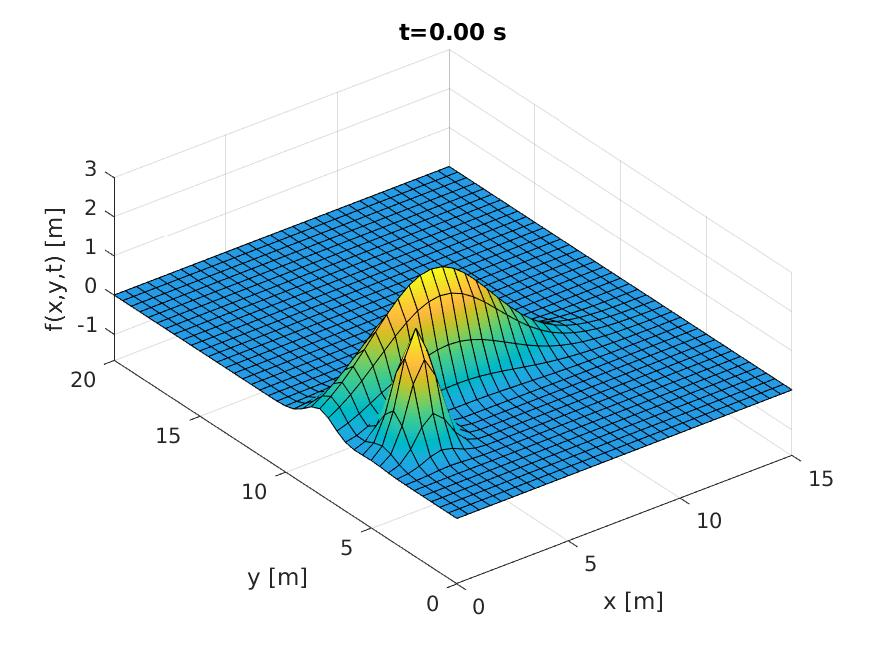
\includegraphics[width=0.495\linewidth,angle=0]{2d/vague_2d_1}
    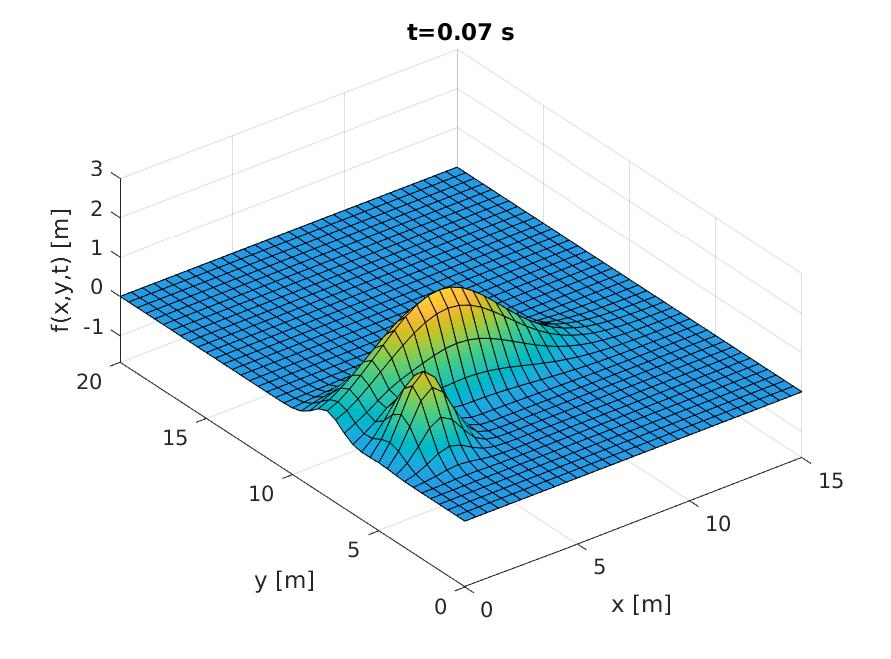
\includegraphics[width=0.495\linewidth,angle=0]{2d/vague_2d_10}
    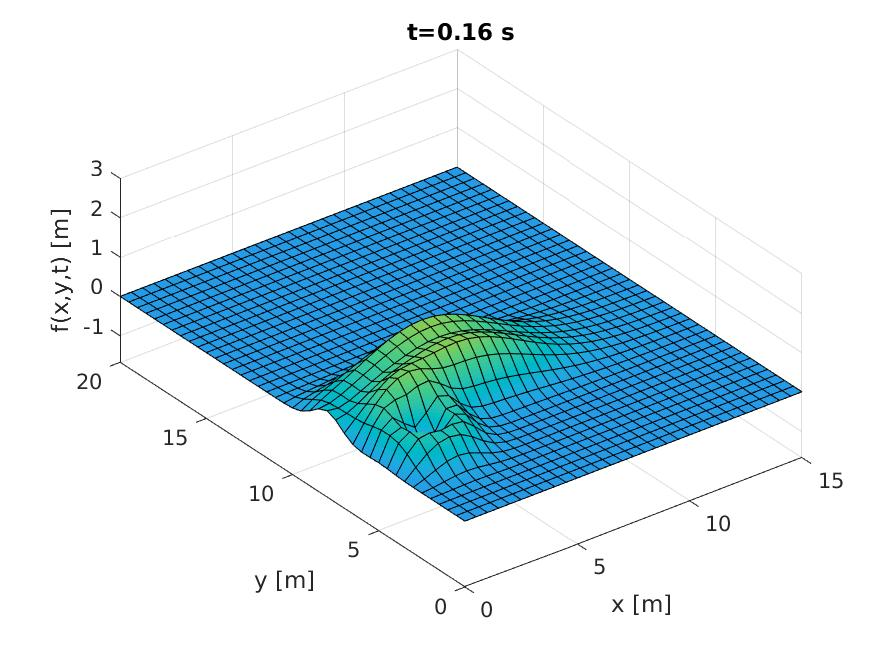
\includegraphics[width=0.495\linewidth,angle=0]{2d/vague_2d_20}
    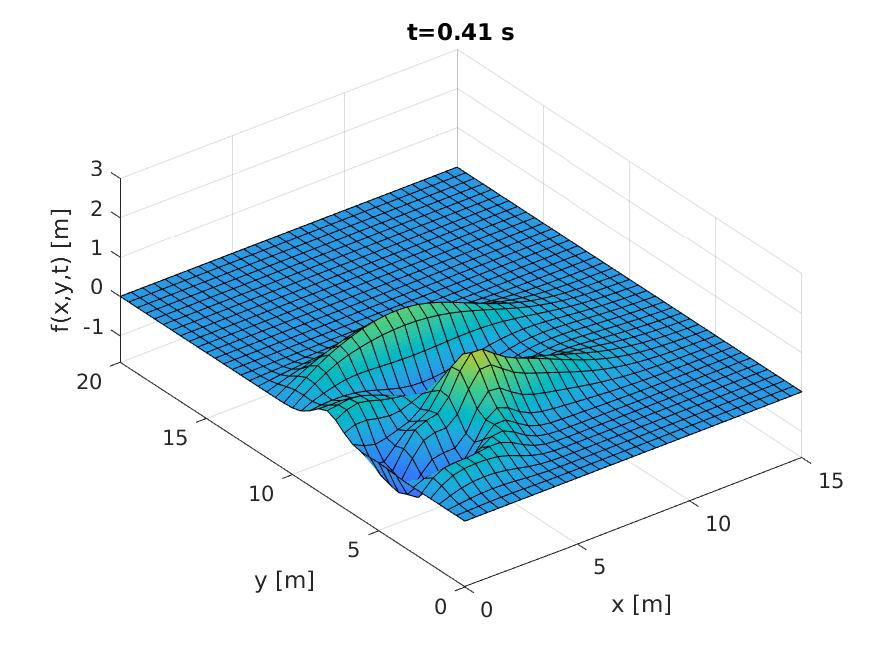
\includegraphics[width=0.495\linewidth,angle=0]{2d/vague_2d_50}
    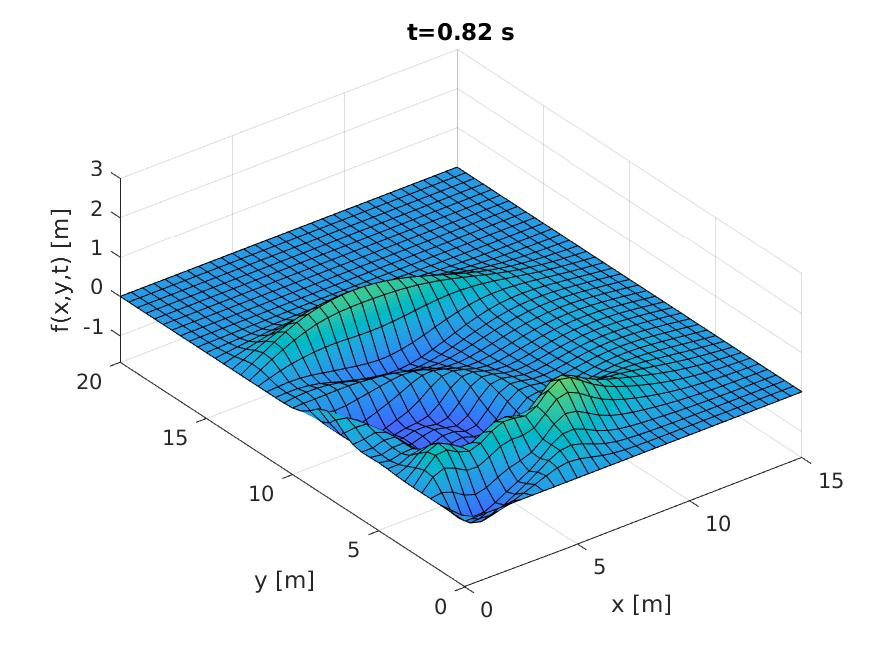
\includegraphics[width=0.495\linewidth,angle=0]{2d/vague_2d_100}
    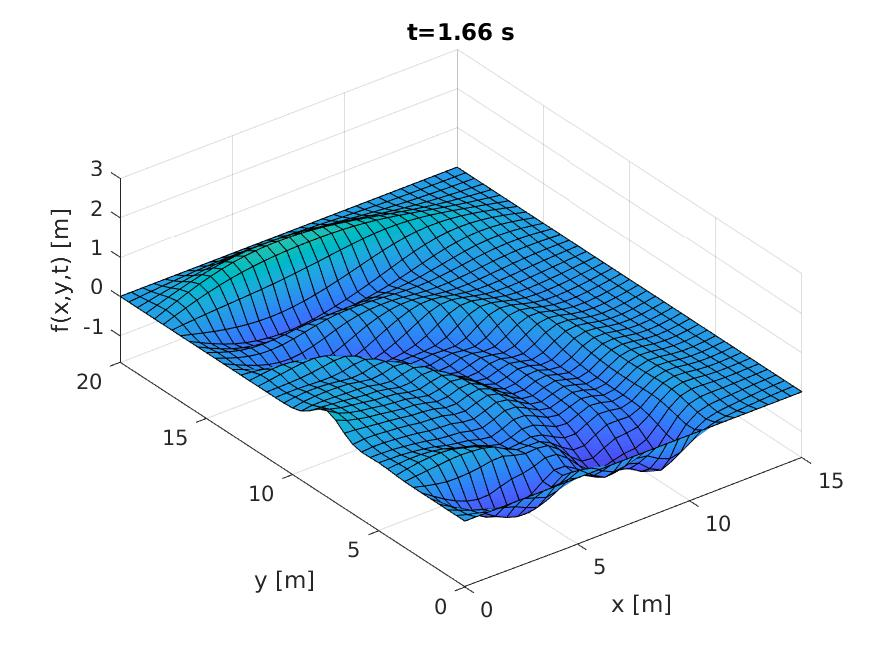
\includegraphics[width=0.495\linewidth,angle=0]{2d/vague_2d_200}
    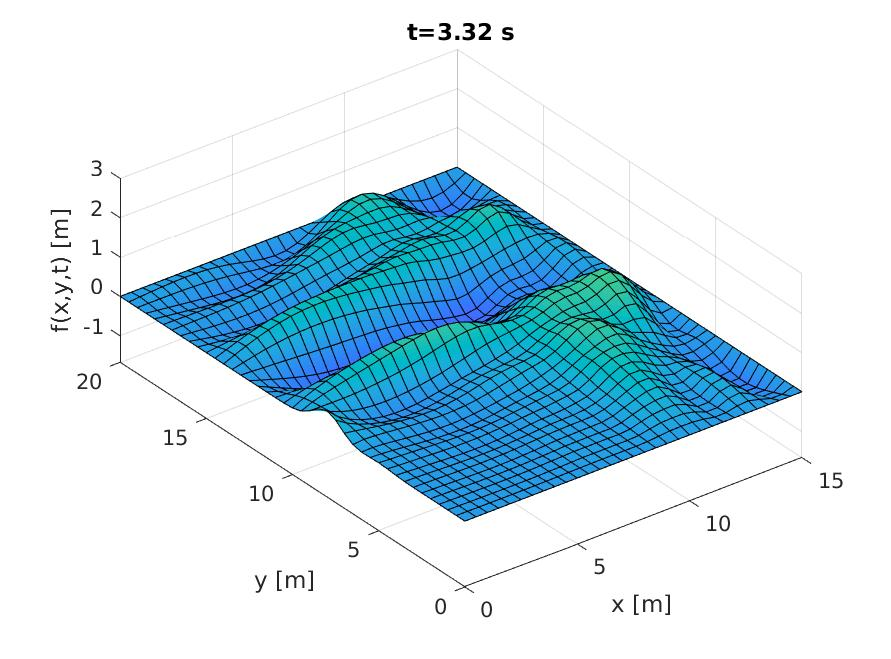
\includegraphics[width=0.495\linewidth,angle=0]{2d/vague_2d_400}
    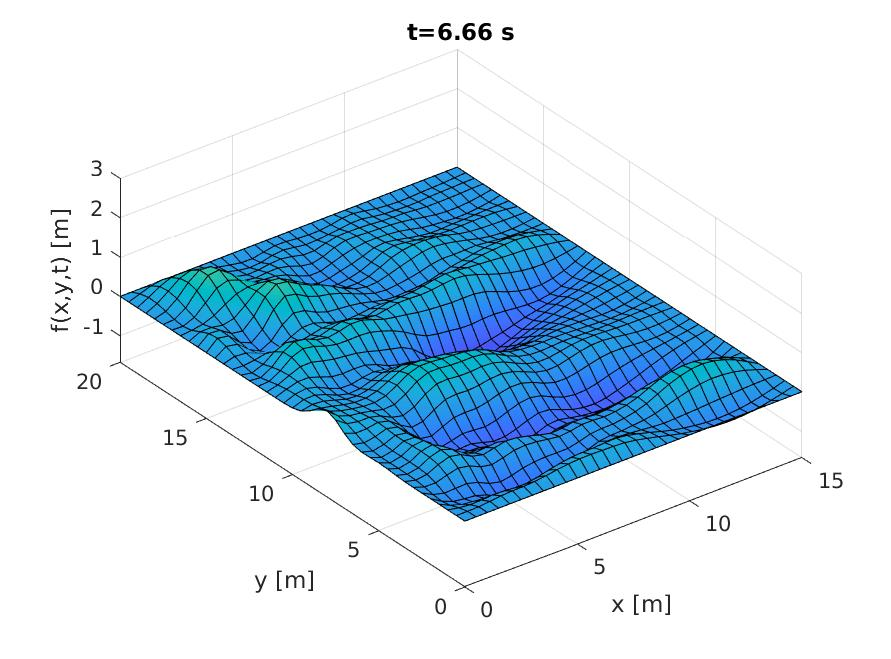
\includegraphics[width=0.495\linewidth,angle=0]{2d/vague_2d_800}
    \caption{Simulation en deux dimensions avec condition de bord fixe.}
    \label{fig:cfl_scan}
\end{figure}

%%%%%%%%%%%%%%%%%%%%%%%%%%%%%%%%%%%%%%%%%%%%%%%%%%%%%%%%%%%%%%%%%%%%%%%%%%%%%%%%%%%%%%%%%%%%%%%%%%%%%%%%
\section{Conclusion}
Dans cet exercice, nous avons pu étudier la propagation d'ondes dans un milieu unidimensionnel à vitesse de propagation variable. Nous avons vérifier dans premier temps que nos schémas étaient corrects pour une vitesse de propagation constante, où des solutions analytiques ont pu être calculées et comparées avec nos résultats numériques. Une fois cette vérification passée avec succès, nous avons étudié le comportement des trois équations proposées dans le cas d'une vitesse de propagation variable Nous avons pu obtenir numériquement l'évolution d'une vague passant par un récif, ce qui n'est pas possible analytiquement, démontrant une nouvelle fois l'utilité des méthodes numériques.


\begin{thebibliography}{99}
\bibitem{donneeEX7} 
Donnée de l'exercice 7. Laurent Villard, EPFL, 2019.
\bibitem{notesDeCours}
Physique numérique I/II, notes de cours. Laurent Villard, EPFL, 2018.
\end{thebibliography}

\end{document} 